\chapter{Diage Modelling Language}
\label{ch:dml}
To help me visualise the stories I wanted to tell within Rouge, I needed a tool in which I could quickly draw up a narrative scenario to test different operators that the Narrator would perform.
For this purpose I developed the Diage Modeling Language, or DML. 
DML is a very simple modeling language akin to those found in the UML specification.
With DML I could create a scenario and declare certain operators to create a finite amount of possible story outcomes. 
It served it's usage as a prototyping tool and set the benchmark for what would become the Narrator.

Some functionalities that Rouge has were not conceived yet during the development of DML. The most noticeable are the actor attributes.
That system was brought into the Narrator after the half way point of research and development time, in which DML was not actively used any more.

DML served its purpose for the early development phase by allowing me a quick and easy way to set up story prototypes, define the working operators that a narrative planner could use, and discover what kind of variations a - then hypothetical - planner could come up with.

This chapter serves as a run down of the DML specification, listing the applications and possible future work relating to it.

\section{The structure of DML}
DML is structured with the use of entities.
These entities in three forms; \code{Actors}, \code{Objects}, and \code{Spaces}.
The latter is also an information container which I will discuss in section~\ref{sec:informationcontainers}.
The following section will only cover the entities that affect the story directly; the objects and actors.
In conjunction with \code{actions} and \code{accessors} these entities convey story information and plot progression.

\begin{figure}[h]
	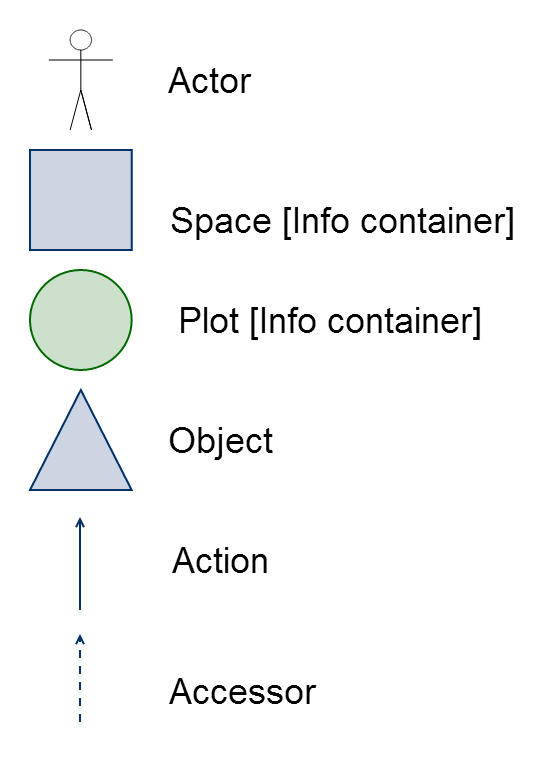
\includegraphics[scale=.5]{symbols}
	\caption{DML Symbols}
	\label{fig:DMLSymbols}	
\end{figure}


\subsection{Objects}
\diage objects form the basis of all entities.
They represent the props and items that we find in the world that have narrative importance.
For example; if the Player walks into a shop, \diage does not specify all items that one could buy in the shop, but only those that have plot importance.
In terms, these objects should adhere to the \textit{Checkhov's Gun} principle.
This dramatic principle states that all objects used in a narrative should eventually be used.
I quote: "\textit{One must never place a loaded rifle on the stage if it isn't going to go off.
It's wrong to make promises you don't mean to keep.\footnote{\url{http://berlin.wolf.ox.ac.uk/lists/quotations/quotations_by_ib.html}}}"
Objects have three properties; a \code{name}, a \code{ID} and a \code{type} The ID is a unique identifier dependant on the type.
And the type is used with actions/accessors as seen in figure~\ref{fig:actions} (Futher discussed in section~\ref{sec:actors}).
The name is the noun given to an object within the story context.
For example; The player receives the \textit{Skeleton Key of Awesomeness}, but the type is just \code{key} giving it no special properties than any other key.
It might make sense to name an object something else than it's type, but a name is not given it defaults to it's type.

Objects form the world, and all other entities derive from the \diage object.
This means that all entities have the same properties as the object, but can extend upon it.
\subsection{Actors}
\label{sec:actors}
An actor is the representation of any one object that can, as the noun implies, act.
Examples are the store-clerk, a wandering adventurer or the player.
The actor is the only entity that can physically interact with the world, and by doing so the only that can change the world's state.
By being able to change the world, the actors are the only entities that can ensure plot progression.

Just like the object, an actor has three properties; a \code{name}, a \code{ID} and a \code{type}.
The type property is used in predefined actions as seen in figure~\ref{fig:actions:npc}.
This figure defines that the \code{Player} can \textbf{speak} to all actors of type \code{NPC}.
A further glance at figure~\ref{fig:actions} shows some more actions that could be defined for the player actor.
These predefined actions tell us that the player can trigger all events and enter all spaces.
I will expand upon these actions in section~\ref{sec:actions_and_accessors}.

\section{Spaces}
\label{sec:informationcontainers}
Information containers are entities that hold story information.
A space holds information about its spacial children Information containers have the unique property that they are nestable.
For example; a space that represents a city can hold several spaces that represents housing.


A space is the representation of any segment of the world or the world itself.
As spaces are info containers they are nestable, as mentioned before, but they differ in the fact that they can hold every entity as a child.
These children make up the spacial awareness of the space and tells us what information it can pass on to actors.
Usually an actor gains all the information a space can give upon the moment it enters the space; when the actor becomes a child object to the space.
This can be modified, and some parts of information maybe withheld from the actor, but this is where the events come in.

\section{Actions and Accessors}
\label{sec:actions_and_accessors}
Actions and accessors are the abstract connectors in \diage.
They convey what actors can do (actions) and what knowledge they possess (accessors).
Some accessors are implied, due to the fact that an actor might be the child of a space, in other cases these connections are explicitly added to a \diage model.
If we review the diagram in figure~\ref{fig:examplediagram} we see that the Mayor has no connections whatsoever.
This would imply that the Mayor has no knowledge about what's or who's in the store.
If we compare figure~\ref{fig:examplediagram} to figure~\ref{fig:example:accessors}, we see that the Mayor now has a connection to the Shop, thus we can be sure that the Mayor has the knowledge it would have, if it had been in the shop space itself.

\begin{figure}[ht]
	\centering
	\begin{subfigure}[b]{0.3\textwidth}
		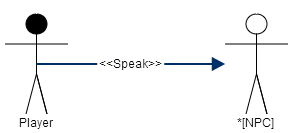
\includegraphics[width=\textwidth]{npc_action}
		\caption{A standard action for NPC interaction}\label{fig:actions:npc}
	\end{subfigure}
	\begin{subfigure}[b]{0.3\textwidth}
		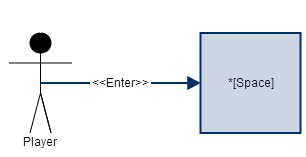
\includegraphics[width=\textwidth]{space_action}
		\caption{A standard action for space interaction}\label{fig:actions:space}
	\end{subfigure}
	\caption{Predefined actions}\label{fig:actions}
\end{figure}

\begin{figure}[ht]
	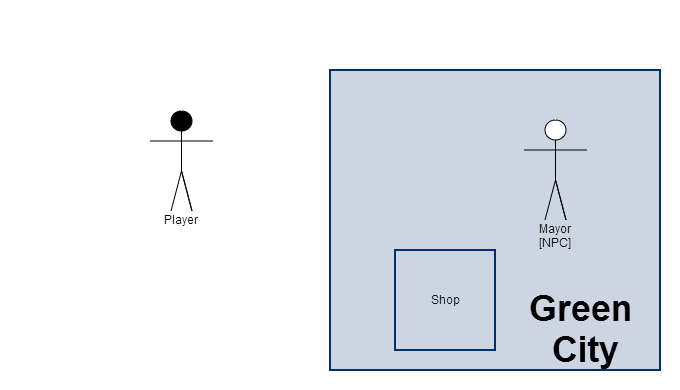
\includegraphics[scale=.5]{diagram_actor_example}
	\caption{An example of a Diage diagram using predefined actions}\label{fig:examplediagram}
\end{figure}
\begin{figure}
	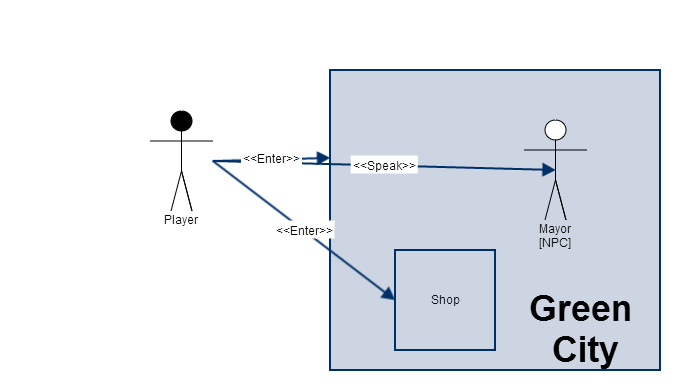
\includegraphics[scale=.5]{diagram_actor_example_verbose}
	\caption{An example of a Diage diagram without using predefined actions}\label{fig:examplediagramverbose}
\end{figure}
\begin{figure}
	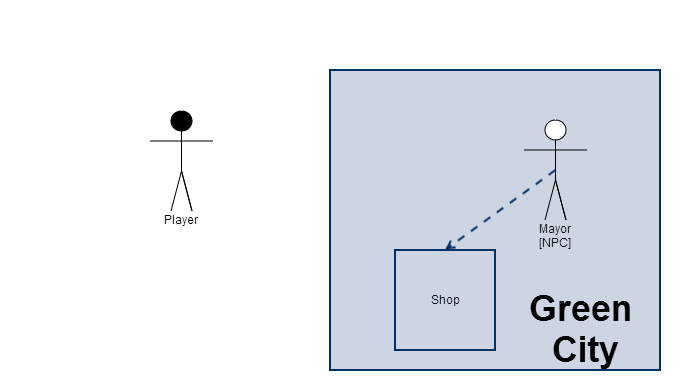
\includegraphics[scale=.5]{diagram_accessor_example}
	\caption{A \diage diagram showing a explicit connection between the Mayor and the Shop}
	\label{fig:example:accessors}
	
\end{figure}

\section{The narration}	
A DML diagram is a snapshot of the current narrative setting, and displays all relevant information to that setting.
One look at the diagram should tell you what a given entity knows about its surroundings.
This information can be conveyed whenever a entity interacts with an other entity.

As a rule, only actors are allowed to record information.
Objects are still-lives and as such do not have spacial awareness, but may give information to the actor.
The prime example is a treasure map that an actor picked up.
The object in question contains the information on a possible treasure as located by the map.
This information gets transferred the same way that an actor could learn new information from another actor.

As a snapshot of the given scene, DML loses the information of the scenario's before and after it. To gain a sense of story progression, one needs to look at several diagrams in quick succession to see what is really happening. Observe figures \ref{fig:narrative} and \ref{fig:narrative2}. These two diagrams display how a story segment (or quest in this instance) is modelled in DML. The examples in question are of the \textit{Save the Princess} and \textit{Fetch} quest variety. 

\begin{figure}[h]
	\centering
	\begin{subfigure}[b]{0.4\textwidth}
		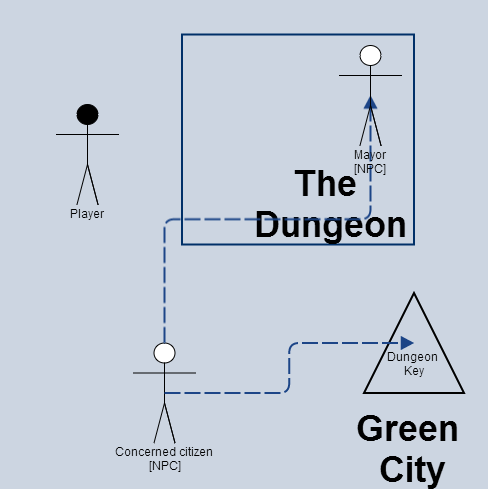
\includegraphics[width=\textwidth]{narrative/1}
		\caption{Initial state.}\label{fig:narrative:1}
	\end{subfigure}
		~
	\begin{subfigure}[b]{0.4\textwidth}
		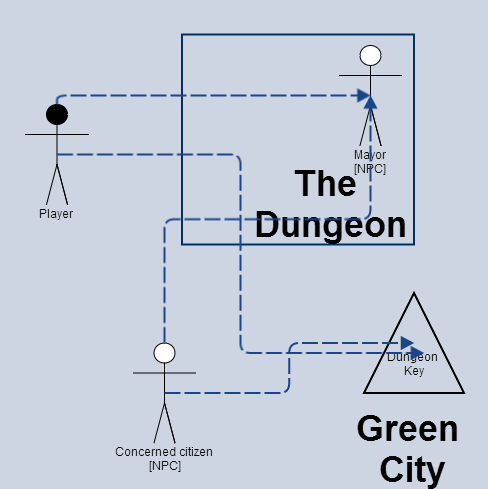
\includegraphics[width=\textwidth]{narrative/2}
		\caption{Player speaks to the NPC}\label{fig:narrative:2}
	\end{subfigure}
		~
	\begin{subfigure}[b]{0.4\textwidth}
		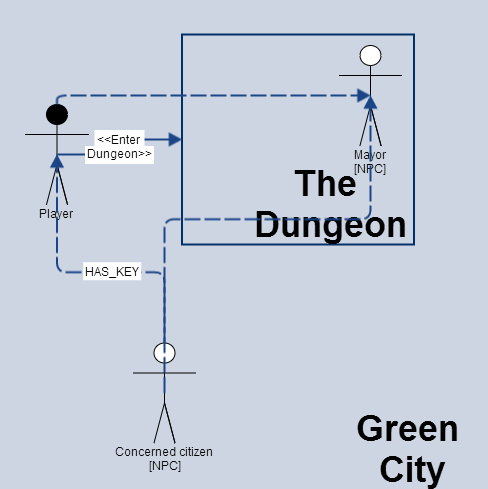
\includegraphics[width=\textwidth]{narrative/3}
		\caption{Player has aquired the key}\label{fig:narrative:3}
	\end{subfigure}
		~
	\begin{subfigure}[b]{0.4\textwidth}
		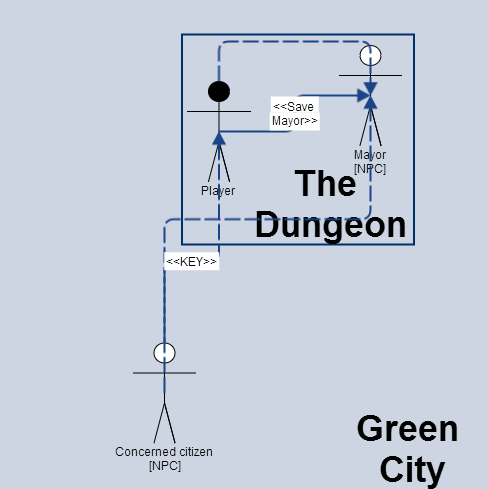
\includegraphics[width=\textwidth]{narrative/4}
		\caption{The player entered the dungeon to save the \textit{Mayor}}\label{fig:narrative:4}
	\end{subfigure}
	~
	\begin{subfigure}[b]{0.4\textwidth}
		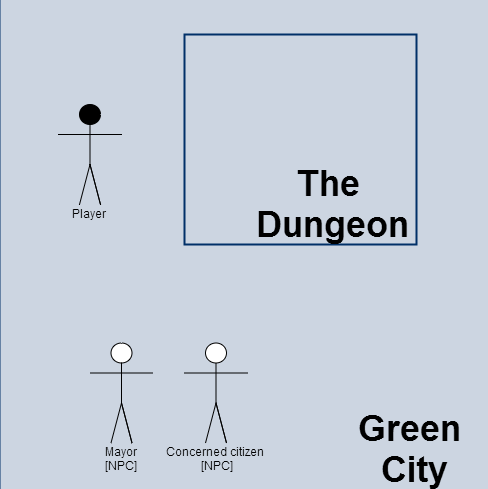
\includegraphics[width=\textwidth]{narrative/5}
		\caption{The mayor is rescued from the dungeon! You stallwart hero of the land!}\label{fig:narrative:5}
	\end{subfigure}
	\caption{A \textit{Save the Princess} quest modelled in DML}\label{fig:narrative}
\end{figure}

The five diagrams in figure~\ref{fig:narrative} shows us a \textit{Save the Princess} quest. The Mayor is trapped, and the concerned citizen asks the player for help. To get into the dungeon the player needs the dungeon key, and helpfully the citizen told him where he could find that key. After unlocking and entering the dungeon, the player will have found the mayor in some kind of distressful state, and leads him outside.
The point is, that we need the knowledge of previous story states, before we can assume that we know what is happening. 
DML has not been designed as a language that tells a story, but purely a way to display the state of one at a certain point of time.

\begin{figure}[h]
	\centering
	\begin{subfigure}[b]{0.4\textwidth}
		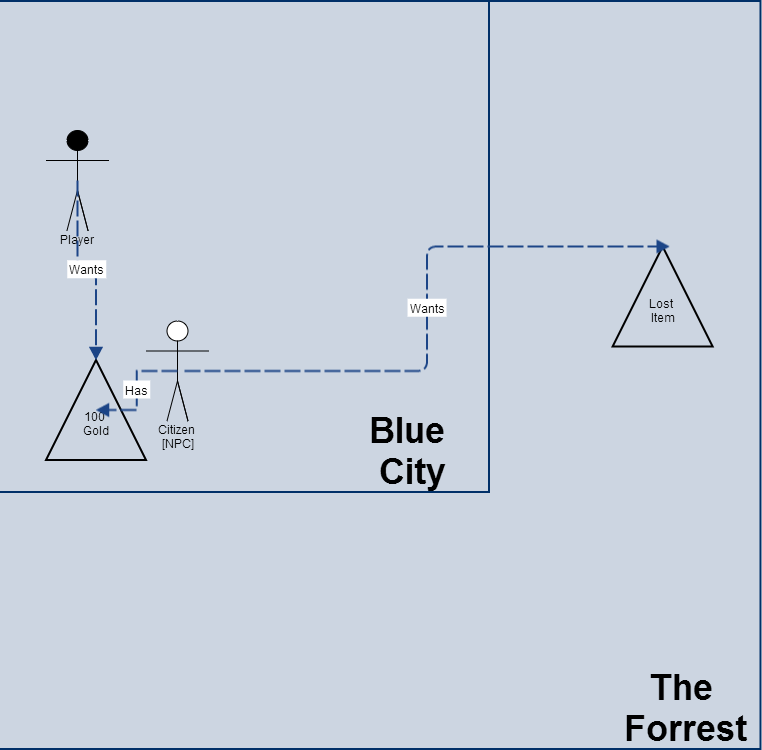
\includegraphics[width=\textwidth]{narrative/2-1}
		\caption{Initial state.}\label{fig:narrative2:1}
	\end{subfigure}
		~
	\begin{subfigure}[b]{0.4\textwidth}
		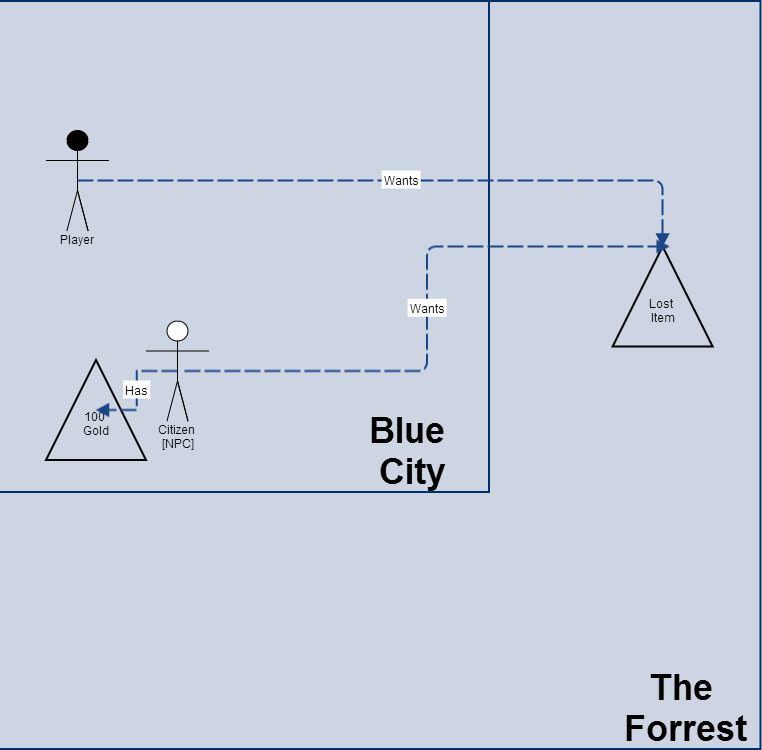
\includegraphics[width=\textwidth]{narrative/2-2}
		\caption{The player speaks to the NPC}\label{fig:narrative2:2}
	\end{subfigure}
		~
	\begin{subfigure}[b]{0.4\textwidth}
		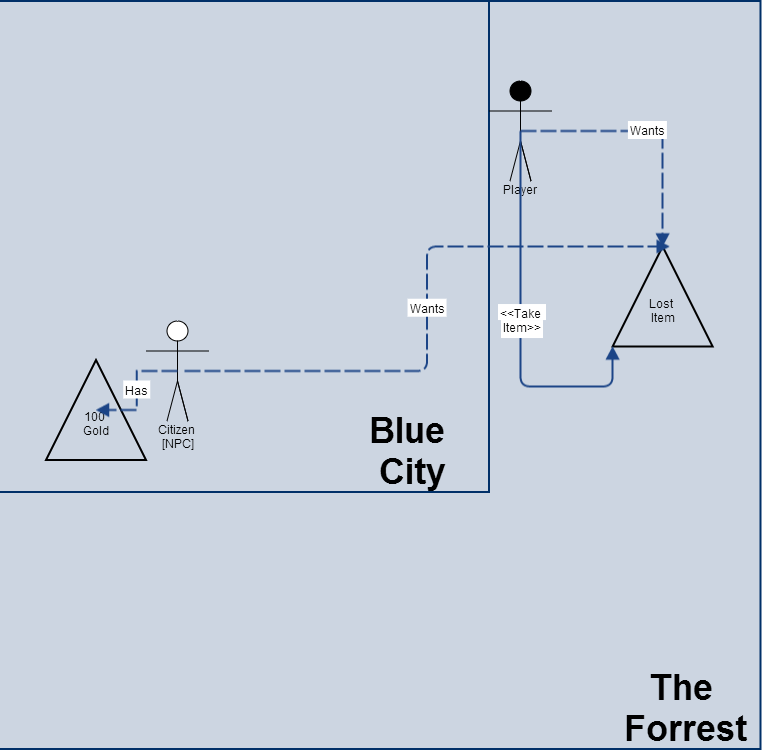
\includegraphics[width=\textwidth]{narrative/2-3}
		\caption{The player enteres the forrest to retrieve the lost item.}\label{fig:narrative:2:3}
	\end{subfigure}
		~
	\begin{subfigure}[b]{0.4\textwidth}
		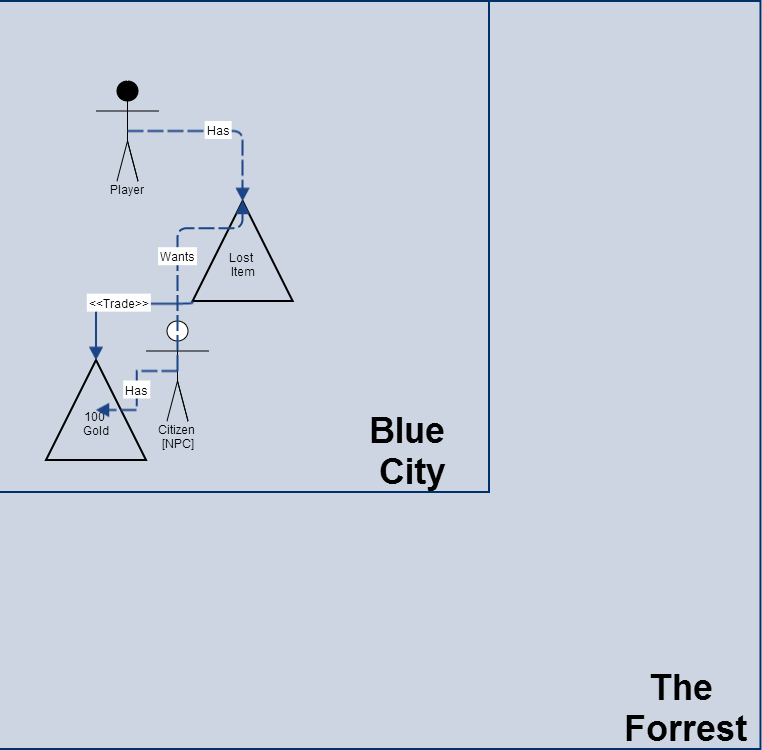
\includegraphics[width=\textwidth]{narrative/2-4}
		\caption{The player returned to the city with the lost item.}\label{fig:narrative2:4}
	\end{subfigure}
		~
	\begin{subfigure}[b]{0.4\textwidth}
		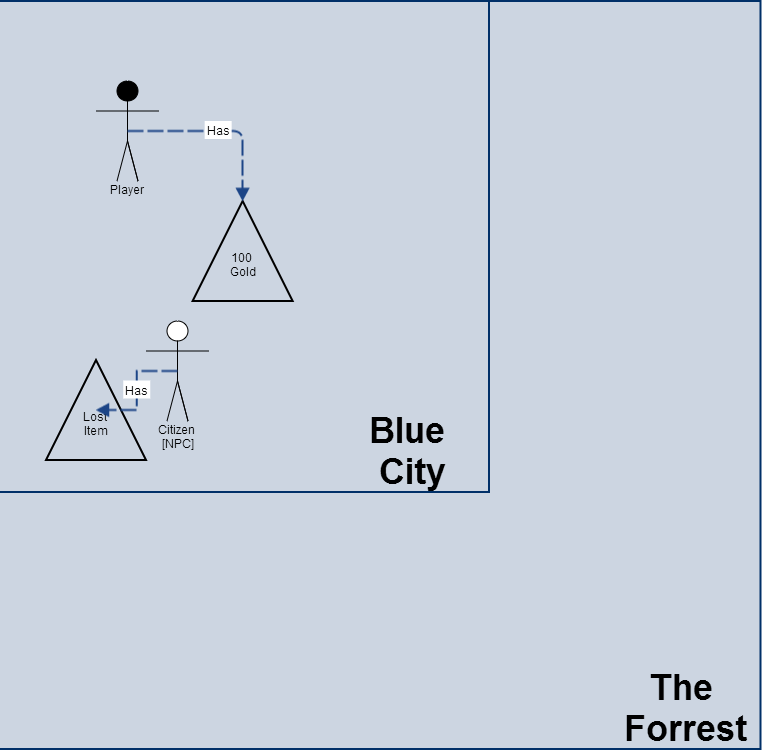
\includegraphics[width=\textwidth]{narrative/2-5}
		\caption{The player traded the item for 100 gold}\label{fig:narrative2:5}
	\end{subfigure}
	\caption{A \textit{Fetch} quest modelled in DML}\label{fig:narrative2}
\end{figure}

Figure~\ref{fig:narrative2} shows us a \textit{Fetch} quest. 
In this quest, the player wants the hundred gold that the NPC has, but in order to gain that money, the player must locate and return an item that the NPC lost in the forest.
Finding and returning said item gives the player the option of trading the lost item for the gold. 

\section{DML in Rouge}
DML was created as tool to help designing and developing the narrative planner, not to be implemented within the game itself. 
However, the possibility of feeding Rouge the initial story state and reviewing the subsequent states that followed was a powerful addition to have.
Enabling the designer to see if any changes made to the Narrator's constraints would have the desired effect, contrasted to outputting a debug log or text dump that could very well be filled with irrelevant information.
The graphing software used up to this point, and indeed for this document, generates files that makes sense for it's type of software; but not to be intelligible for Rouge or the narrative planner.
Hence, the DML Creator was developed.
This tool, as seen in figure~\ref{fig:DMLC:screens}, allows a user to create DML diagrams, add attributes to actors and load the output file in to Rouge.
When the player takes a snapshot of the story state, Rouge creates a similar DML file that the DML Creator can read. 

\begin{figure}
	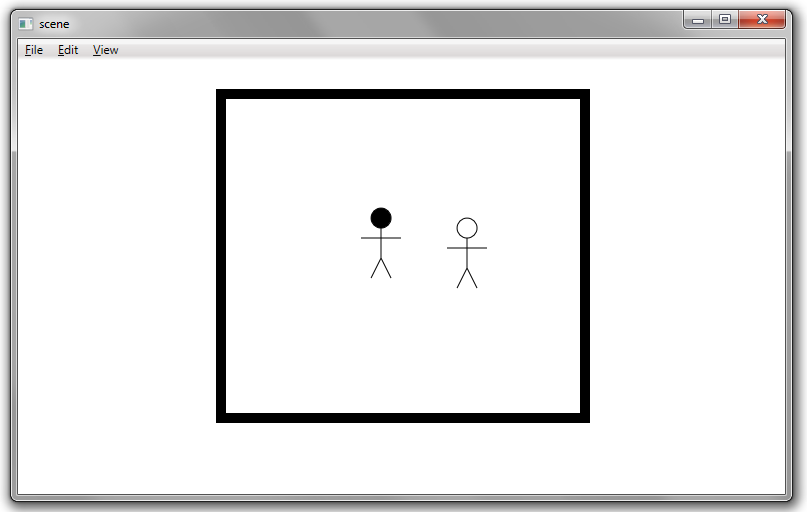
\includegraphics[width=\textwidth]{DMLC/example}
\end{figure}
\begin{figure}
\centering
\begin{subfigure}{0.4\textwidth}
	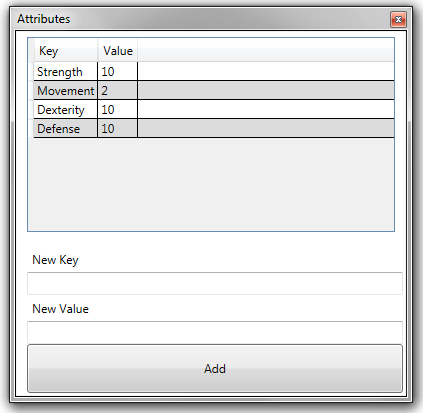
\includegraphics[width=\textwidth]{DMLC/attributes}
\label{fig:DMLC:screens:attributes}
\end{subfigure}
~
\begin{subfigure}{0.4\textwidth}
	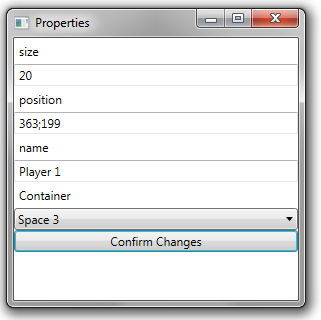
\includegraphics[width=\textwidth]{DMLC/properties}
\label{fig:DMLC:screens:properties}
\end{subfigure}
	\caption{The properties and attribute windows}\label{fig:DMLC:screens}
\end{figure}


\section{Future work}
\diage is normally expressed with a DML diagram, but the underlying structure is that of a graph.
Due to time constraints there has been no work done in using this graph as a means to structure the direction of a narrative; however, DML is directly translatable to a graph.
Figure~\ref{fig:graph:fetch} demonstrates this in relation to figure~\ref{fig:narrative2}.
More research in respect to graph translations in relation to \diage could result in a better way to direct the narrative into a specific direction.
As example; the designer could define an initial state, and an eventual state.
Using graph translations \diage could interpolate several \textit{in-between} states that the narrative will take as seen in figure~\ref{fig:graph}.
A method could be developed in which \diage could output all variants of narrative trees respectively to the choices available to the player, displaying all possible endings a discreet story arc could have.

\begin{figure}
\centering
	\begin{subfigure}{0.4\textwidth}
		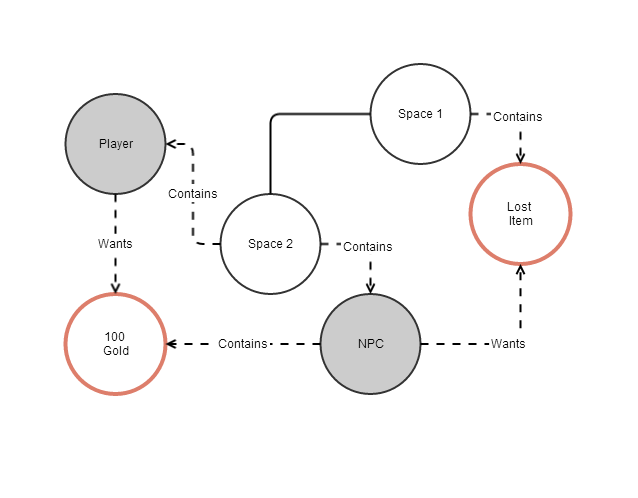
\includegraphics[width=\textwidth]{graph/ex-1}
	\end{subfigure}
	\begin{subfigure}{0.4\textwidth}
		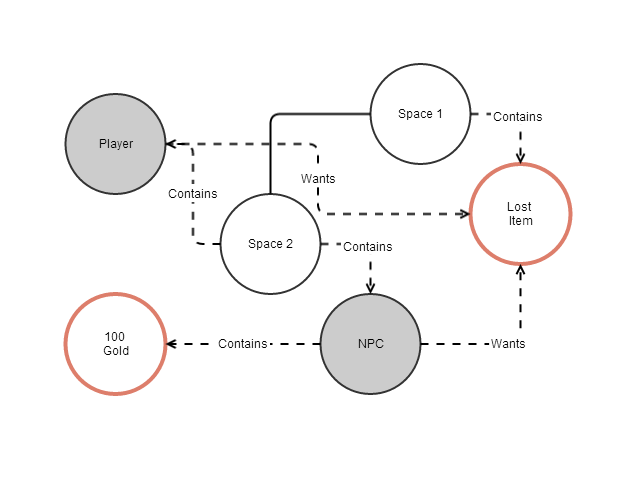
\includegraphics[width=\textwidth]{graph/ex-2}
	\end{subfigure}
	\begin{subfigure}{0.4\textwidth}
		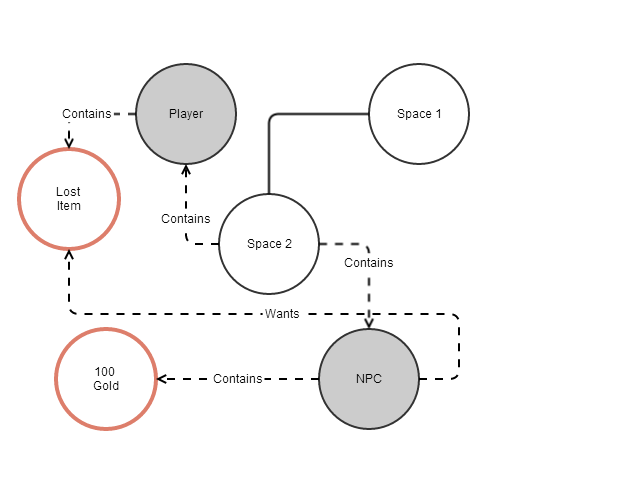
\includegraphics[width=\textwidth]{graph/ex-3}
	\end{subfigure}
	\begin{subfigure}{0.4\textwidth}
		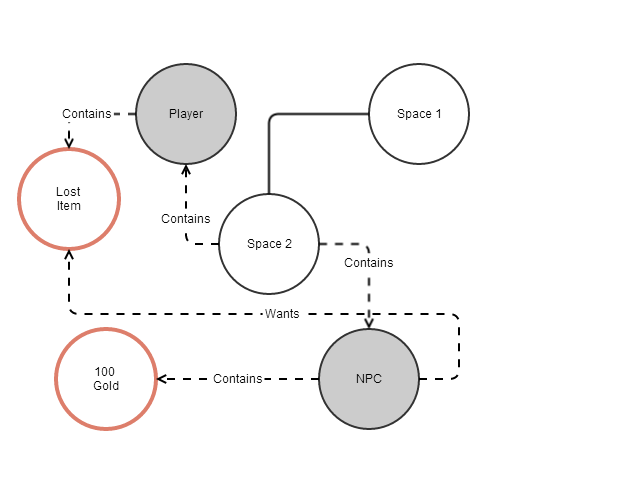
\includegraphics[width=\textwidth]{graph/ex-4}
	\end{subfigure}
	\begin{subfigure}{0.4\textwidth}
		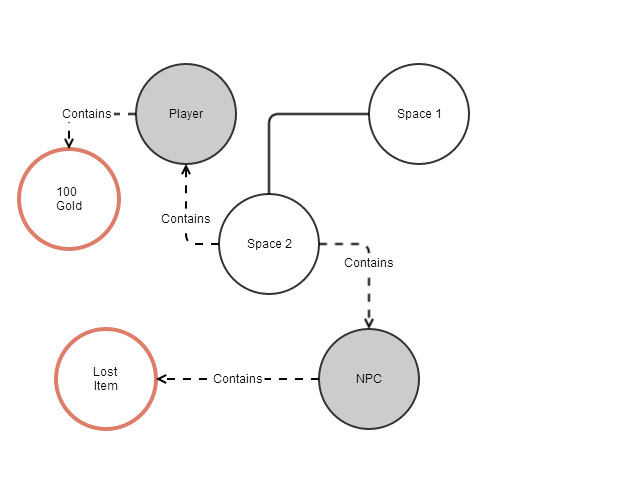
\includegraphics[width=\textwidth]{graph/ex-5}
	\end{subfigure}
	\caption{Figure~\ref{fig:narrative2} represented as a graph}\label{fig:graph:fetch}
\end{figure}

\begin{figure}
	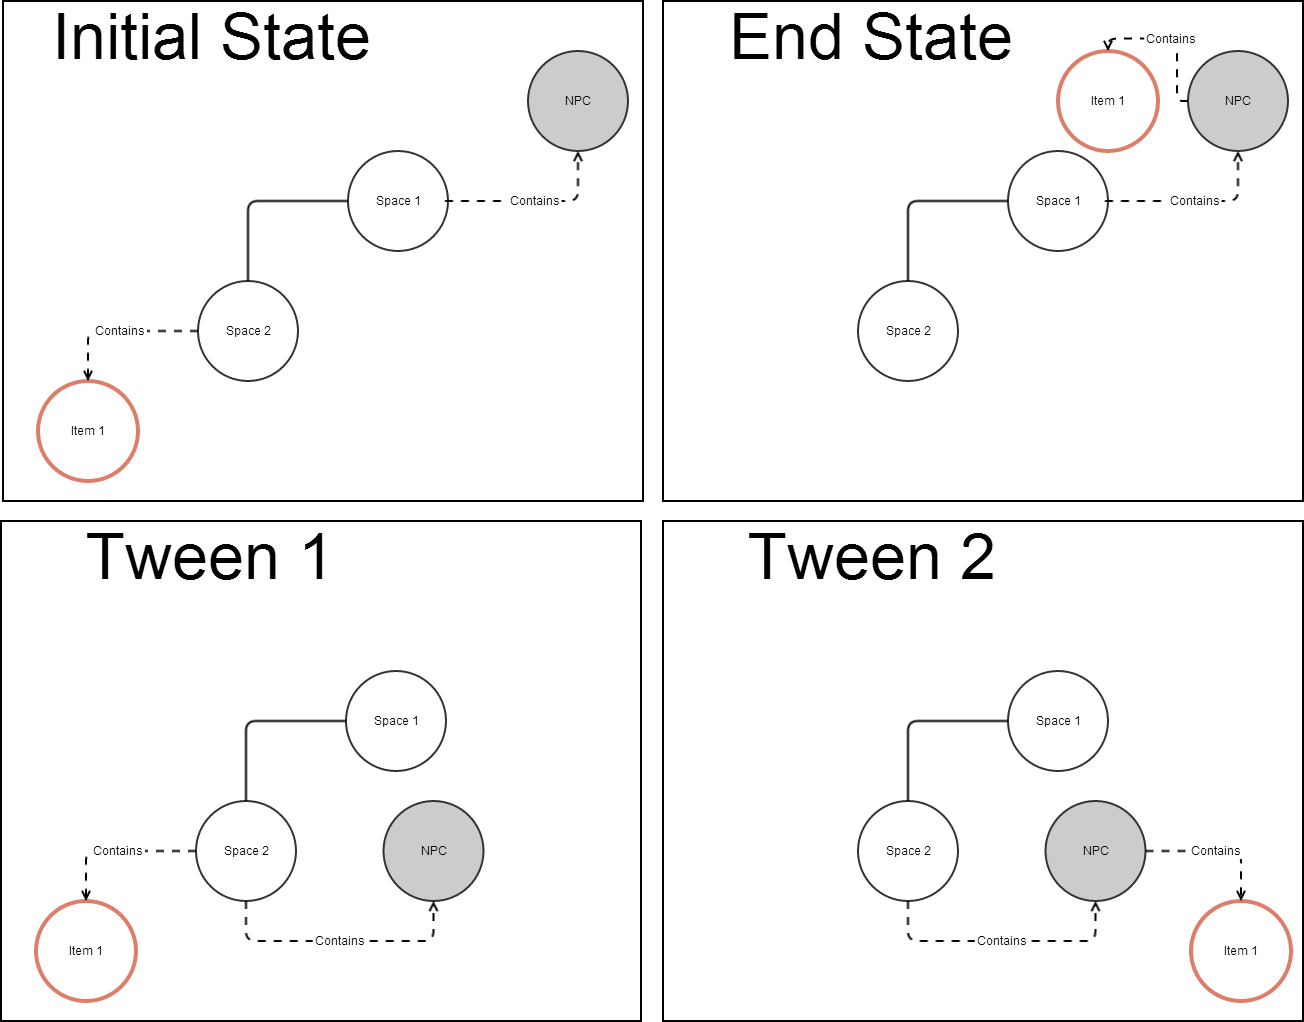
\includegraphics[width=\textwidth]{graph/total}
	\caption{An example of an interpolated graph} \label{fig:graph}
\end{figure}
